\documentclass[crop,class=article]{standalone}
%----------------------------Preamble-------------------------------%
\usepackage{tikz}                       % Drawing/graphing tools.
\usetikzlibrary{arrows.meta}            % Latex and Stealth arrows.
%--------------------------Main Document----------------------------%
\begin{document}
    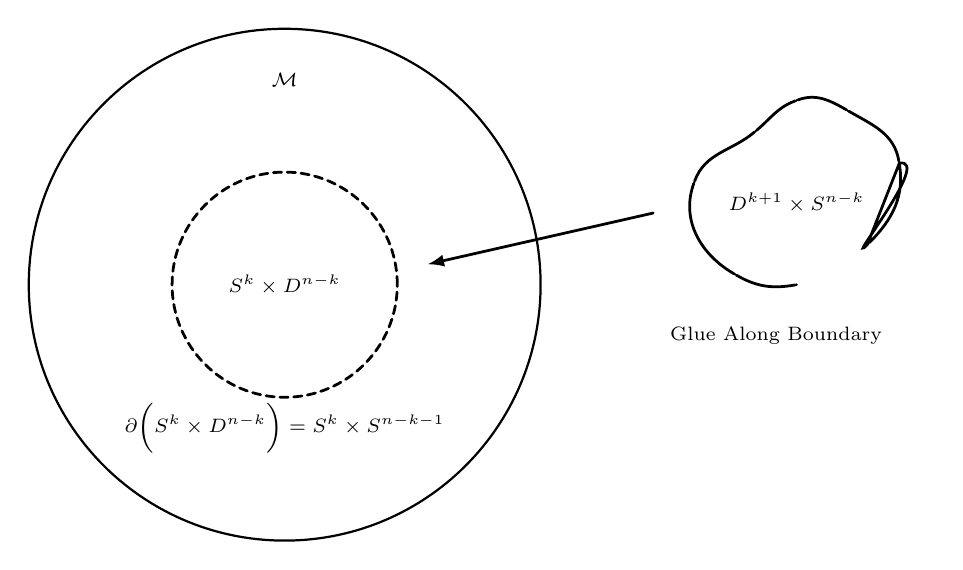
\begin{tikzpicture}[%
        font=\scriptsize,
        scale=1.3,
        line width=1pt,
        line cap=round,
        >={Latex[black]},
        every edge/.style={draw=black,very thick}
    ]
        \draw[densely dashed] (0,0) circle (1.1);
        \draw[thick] (0,0) circle (2.5);
        \node at (0,2) {$\mathcal{M}$};
        \node at (0,0) {$S^{k}\times D^{n-k}$};
        \node at (0,-1.4)
            {
                $\partial\big(S^{k}\times{D^{n-k}}\big)%
                 =S^{k}\times{S^{n-k-1}}$
            };
        \begin{scope}[%
            every node/.style={
                fill=black,
                circle,
                inner sep=0pt,
                outer sep=0pt
            }
        ]
            \node at (5,0) (a) {};
            \node at (4.4,0.1) (b) {};
            \node at (4,1) (c) {};
            \node at (4.6,1.5) (d) {};
            \node at (5, 1.8) (e) {};
            \node at (5.5, 1.7) (f) {};
            \node at (6,1.2) (g) {};
            \node at (5.7,0.4) (h) {};
        \end{scope}
        \node at (5,0.8) {$D^{k+1}\times{S^{n-k}}$};
        \draw[>=latex,->] (3.6,0.7)--(1.4,0.2);
        \node at (4.8,-0.5) {Glue Along Boundary};
        \draw (a) to [out=-170,in=-30] (b)
                  to [out=150,in=-110] (c)
                  to [out=70,in=-140] (d)
                  to [out=40,in=-160] (e)
                  to [out=20,in=150] (f)
                  to [out=-30,in=100] (g)
                  to [out=-80,in=45] (h)
                  to [out=-135,in=10] cycle;
    \end{tikzpicture}
\end{document}